\subsection{Wonder 3D}\label{Wonder3D}

\citeauthor{long2023wonder3d} introduce Wonder3D, a technique that stands apart from its predecessors primarily through its adeptness in generating color images and consistent multi-view normal maps. This method leverages a cross-domain diffusion model, which ``extends the stable diffusion framework to model the joint distribution of two different domains, i.e., normals and colors'' \citep{long2023wonder3d}.


\begin{figure}[ht]
  \centering
    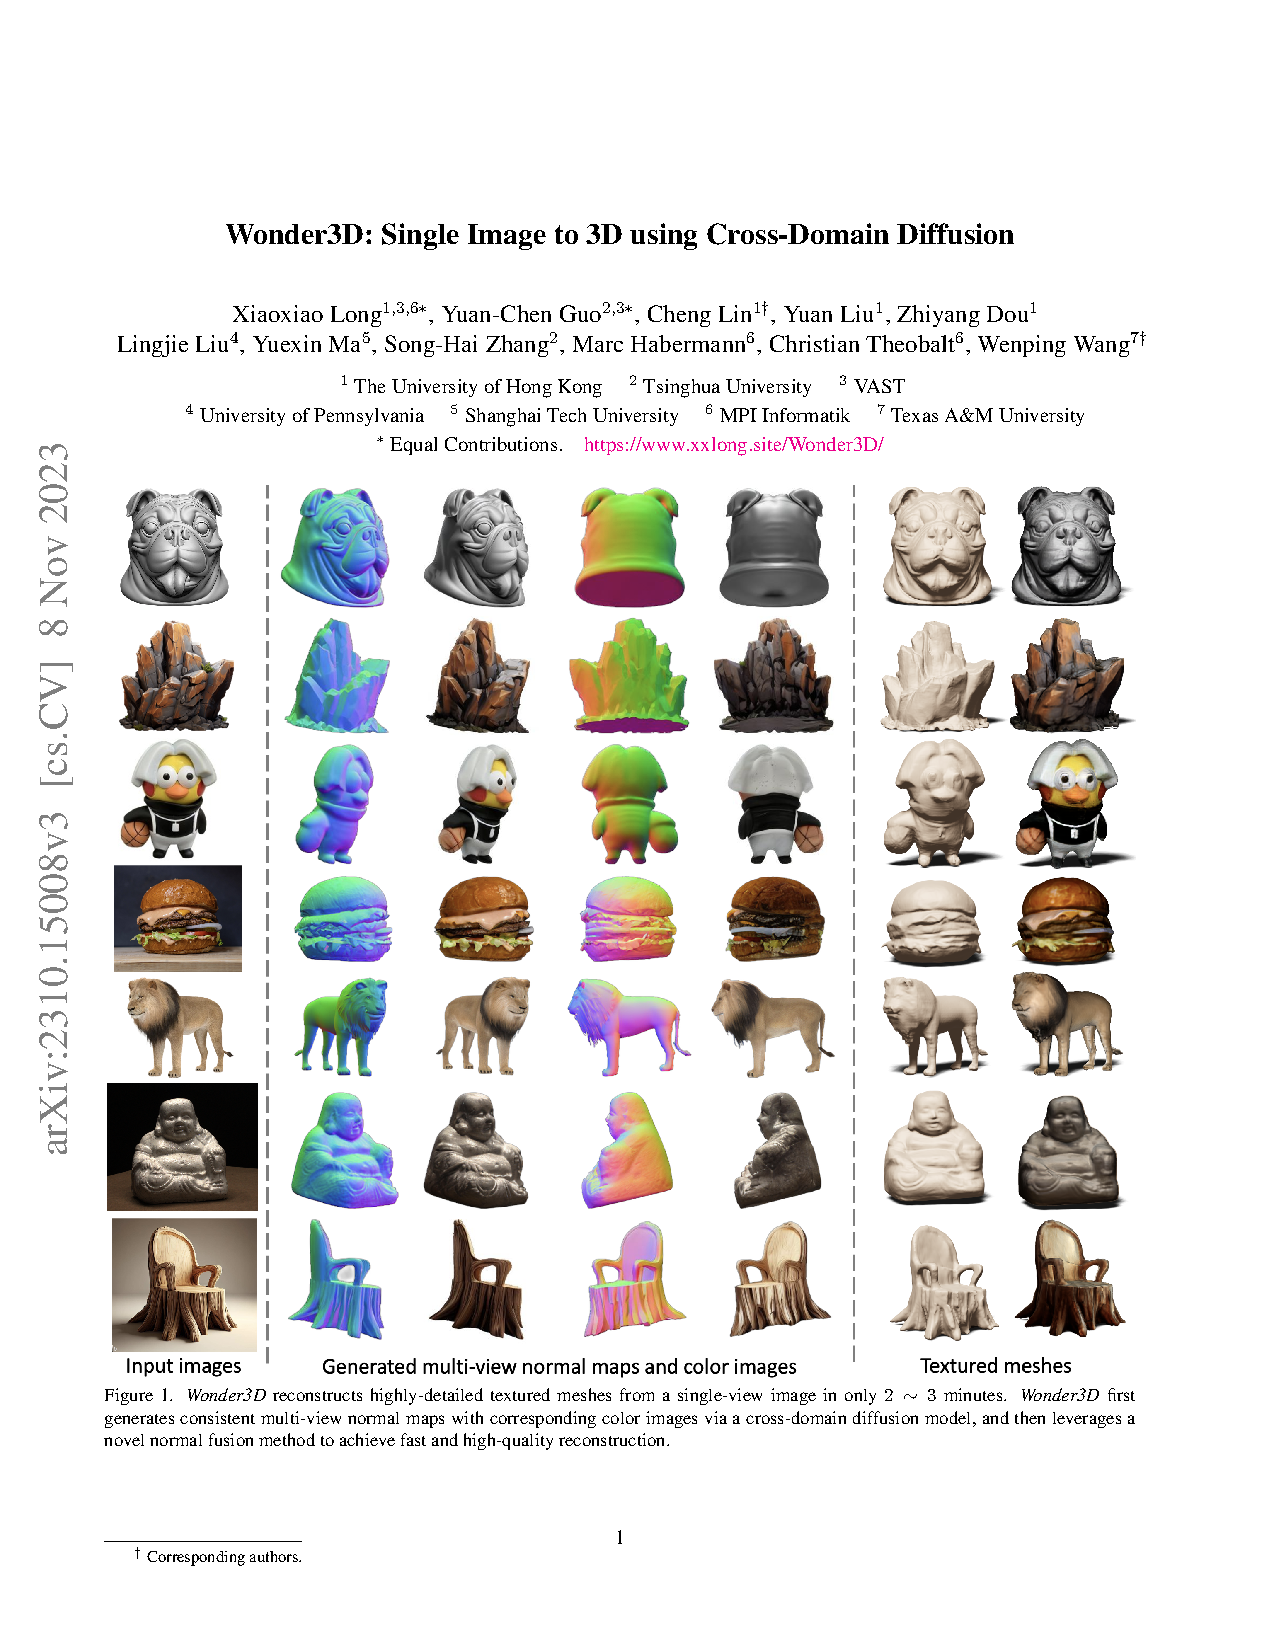
\includegraphics[width=1\columnwidth]{figures/Wonder3D.png}
    \caption{Summarized functionality of Wonder3D, illustrating its unique approach in generating high-fidelity textured meshes from single images using cross-domain diffusion models \citep{long2023wonder3d}.}\label{fig:Wonder3D}
\end{figure}

The process of generating 3D models from images begins with the use of CLIP \citep{radfordCLIP} to obtain a textual description of the image. Wonder3D allows for training on 2D diffusion models by using a unique formulation of 3D models. The distribution of 3D assets is provided ``as a joint distribution of its corresponding 2D multi-view normal maps and color images'' \citep{long2023wonder3d}. 

Given an image \( y \), the model \(f\) aims to produce multiple normal maps \( n^{1:K} \) and color images \( x^{1:K} \) from various camera positions \((\pi_1, \pi_2, \ldots, \pi_k)\), mathematically represented by \citeauthor{long2023wonder3d} as \((n^{1:K}, x^{1:K} | y) = f(y, \pi_{1:k})\).

The creation of the cross-domain joint distribution in Wonder3D is enabled by the use of a Markov chain as part of a diffusion model.~\citeauthor{long2023wonder3d} formally represent this as \[ p\left(n_T^{(1: K)}, x_T^{(1: K)}\right) \prod_t p_\theta\left(n_{t-1}^{(1: K)}, x_{t-1}^{(1: K)} \mid n_t^{(1: K)}, x_t^{(1: K)}\right) \] where \( p\left(n_T^{(1: K)}, x_T^{(1: K)}\right) \) is the Gaussian noise \citep{long2023wonder3d}. For each step \(t\), the model refines the normal maps and color images from the previous step \(t-1\) by refining the model's parameters \(p_\theta\).

Simply adapting pre-trained stable diffusion models to also output both normal maps and color images, encountered issues with slow convergence and poor generalization \citep{long2023wonder3d}. To address these challenges, Wonder3D introduce a cross-domain diffusion scheme named Domain Switcher \(s\), which is given as an extra input to the diffusion model \citep{long2023wonder3d}. \[
  n^{1:K}, x^{1:K} = f(y, \pi_{1:K}, s_n), f(y, \pi_{1:K}, s_c)
\] This equation by \citeauthor{long2023wonder3d} means that the model uses the switcher \( s \) to decide whether to generate normal maps (\( s_n \)) or color images (\( s_c \)), based on the input provided. To ensure geometric consistency between the color image and the normal map for a single view, Wonder3D employs cross-domain attention, allowing for information exchange between multiple domains \citep{long2023wonder3d}.

The transformation from 2D outputs (normal maps and color images) to 3D geometry is achieved by optimizing a neural implicit signed distance field (SDF). This optimization process is geometric-aware, meaning it takes into account the spatial relationships and shapes present in the 2D inputs. This involves segmenting object masks from normal maps or color images, and optimizing by ``randomly sampling a batch of pixels and their corresponding rays in world space [\(\ldots\)]'' \citep{long2023wonder3d}. This method of sampling and adjusting points in the SDF based on the rays ensures that the 3D model is a true representation of the object as seen in the 2D images.

\citeauthor{long2023wonder3d} define the overall objective function as: \[ L = L_{normal} + L_{rgb} + L_{mask} + R_{eik} + R_{sparse} + R_{smooth} \]

Each term serves a specific purpose: \( L_{normal} \) alligns the 3D geometry with the generated normal maps, by employing a cosine function to maximize the similarity between the normals of the signed distance field (SDF) and the generated normals \citep{long2023wonder3d}.~\( L_{rgb} \) ensures color accuracy, and \( L_{mask} \) calculates the errors between masks \citep{long2023wonder3d}. The eikonal regularization term \( R_{eik} \) maintains the stability of the shape, the sparsity regularization term \( R_{sparse} \) avoids isolated and floating parts in the SDF and the smoothness regularization term \( R_{smooth} \) contributes to the natural appearance of the 3D geometry \citep{long2023wonder3d}.

Despite its innovation, Wonder3D has some limitations, as the method can only generate normal and color images from a limited number of six views, which hinders the ability to create intrinsic and finely detailed objects \citep{long2023wonder3d}.  While increasing the number of views could potentially enhance the detail and quality of the output, it would also significantly escalate computational demands \citep{long2023wonder3d}.